\documentclass[10pt,a4paper]{article}

% ============================================================
% PACKAGES
% ============================================================
\usepackage[utf8]{inputenc}
\usepackage[T1]{fontenc}
\usepackage{helvet}
\renewcommand{\familydefault}{\sfdefault}

\usepackage{xcolor}
\usepackage[top=0.7cm,bottom=0.9cm,left=1.0cm,right=1.0cm,footskip=14pt]{geometry}
\usepackage{graphicx}
\usepackage{hyperref}
\usepackage{titlesec}
\usepackage{enumitem}
\usepackage{caption}
\usepackage{booktabs}
\usepackage{fancyhdr}
\usepackage{tabularx}
\usepackage{array}

% ============================================================
% COLOUR PALETTE
% ============================================================
\definecolor{NavyBlue}{RGB}{11,25,44}
\definecolor{SlateBlue}{RGB}{30,62,98}
\definecolor{CyanAccent}{RGB}{14,165,233}
\definecolor{DarkText}{RGB}{30,41,59}

% ============================================================
% PDF METADATA
% ============================================================
\hypersetup{
    colorlinks=true,
    linkcolor=SlateBlue,
    citecolor=SlateBlue,
    urlcolor=CyanAccent,
    pdftitle={MetaRadar - Executive Concept Note},
    pdfauthor={Aura Pharmers}
}

% ============================================================
% HEADER / FOOTER
% ============================================================
\pagestyle{fancy}
\fancyhf{}
\renewcommand{\headrulewidth}{0pt}
\renewcommand{\footrulewidth}{0.4pt}

\fancyfoot[L]{%
    \small\color{DarkText}\textbf{MetaRadar}
    --- Executive Concept Note | Aura Pharmers
}

\fancyfoot[R]{%
    \small\color{DarkText}Page \thepage\ of 2
}

% ============================================================
% SECTION STYLING
% ============================================================
\titleformat{\section}
    {\color{NavyBlue}\small\bfseries}
    {\thesection.}{0.3em}{}
    [\color{CyanAccent}\titlerule]

\titleformat{\subsection}
    {\color{SlateBlue}\scriptsize\bfseries}
    {\thesubsection}{0.3em}{}

\titlespacing*{\section}{0pt}{1.8pt}{1.0pt}
\titlespacing*{\subsection}{0pt}{1.0pt}{0.8pt}

\setlist{
    noitemsep,
    topsep=0.2pt,
    parsep=0.2pt,
    leftmargin=10pt
}

\setlength{\parskip}{0.6pt}
\setlength{\parindent}{0pt}

% Compact figure captions
\captionsetup{
    font=scriptsize,
    labelfont=bf,
    skip=1.0pt
}

% ============================================================
% DOCUMENT
% ============================================================
\begin{document}

% ============================================================
% PAGE 1 — PROBLEM, SOURCES, SOLUTION, FOUR QUESTIONS & ARCHITECTURE
% ============================================================

\fcolorbox{NavyBlue}{NavyBlue}{%
\begin{minipage}{\dimexpr\textwidth-2\fboxsep-2\fboxrule\relax}
\vspace{0.5pt}

{\color{white}\normalsize\bfseries META RADAR\par}

\vspace{0.5pt}

{\color{CyanAccent}\small\bfseries
From Scattered Signals to Strategic Intelligence\par}

\vspace{1pt}

{\color{white}\tiny
\textbf{Team:} Aura Pharmers \quad|\quad
\textbf{Team Lead:} Sanjana Rathore B. \quad|\quad
\textbf{Hackathon:} Novo Nordisk GBS Hackathon 2026 \par
\textbf{Problem Statement \#3:} From Inbox Noise to Strategic Signal
\quad|\quad
\textbf{Pilot Domain:} Haemophilia A \& B (Rare Disease)\par}

\vspace{0.5pt}
\end{minipage}%
}

\vspace{1pt}

% ------------------------------------------------------------
% 1. THE PROBLEM
% ------------------------------------------------------------
\section{The Problem}

The haemophilia treatment landscape is rapidly evolving (non-factor therapies \textit{emicizumab}, \textit{concizumab}, \textit{mim8}; AAV gene therapies \textit{Hemgenix}, \textit{Roctavian}). Critical external signals are fragmented across 8 silos: pharma news, clinical trial registries, scientific publications, medical congresses (ASH, ISTH, WFH), regulatory releases, safety signals, patient/access narratives, and competitor pipeline activity. Cross-functional teams manually find, connect, and interpret these updates. The challenge is turning fragmented external information into actionable intelligence for the right team.

\begin{center}
\vspace{-2pt}
\scriptsize
\textbf{\color{SlateBlue}
Scattered External Sources
$\longrightarrow$
Understand
$\longrightarrow$
Prioritize
$\longrightarrow$
Route
$\longrightarrow$
Act}
\vspace{-2pt}
\end{center}

% ------------------------------------------------------------
% 2. EXTERNAL SIGNAL SOURCES
% ------------------------------------------------------------
\section{External Signal Sources}

MetaRadar monitors a multi-source data landscape categorized across six domains. Primary sources are supported through API connectors in the prototype, supplemented by simulated feeds for extended categories:

\begin{center}
\vspace{-3pt}
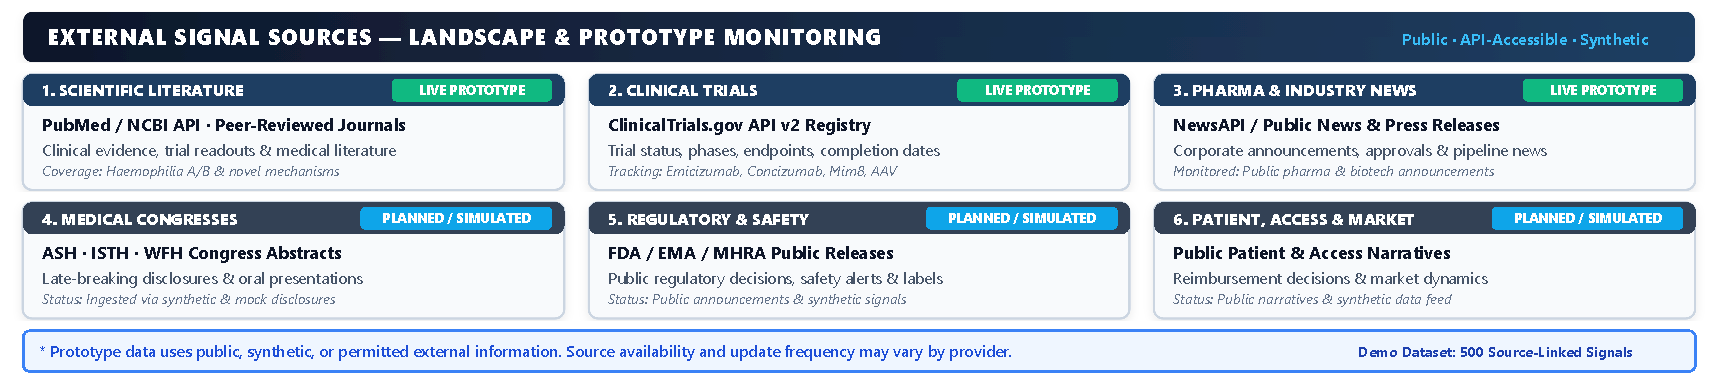
\includegraphics[width=0.96\textwidth]{sources_grid.pdf}
\captionof{figure}{\textbf{External Signal Landscape \& Scope} --- Prototype live connectors explicitly distinguished from planned categories.}
\label{fig:sources}
\end{center}

\vspace{-6pt}

% ------------------------------------------------------------
% 3. OUR SOLUTION
% ------------------------------------------------------------
\section{Our Solution}

\textbf{MetaRadar} is an AI-powered intelligence radar that converts fragmented external haemophilia updates into source-linked, prioritized, explainable, and actionable intelligence. Rather than operating as a generic news dashboard, MetaRadar connects evidence around distinct developments and delivers function-specific insights to six primary Novo Nordisk stakeholders: \textbf{Medical Affairs, Regulatory, Safety / Pharmacovigilance, Market Access, Medical Communications, and Leadership}. Importantly, not every signal is sent to every function; MetaRadar routes each development to the teams most relevant to it.

% ------------------------------------------------------------
% 4. THE FOUR BUSINESS QUESTIONS
% ------------------------------------------------------------
\section{The Four Business Questions}

MetaRadar structures intelligence around four decision-first questions:

\vspace{1pt}

{\scriptsize
\renewcommand{\arraystretch}{1.15}

\begin{tabularx}{\textwidth}{
    |>{\bfseries\color{NavyBlue}\raggedright\arraybackslash}p{4.8cm}|X|
}
\hline
\textbf{\color{NavyBlue}Business Question}
&
\textbf{\color{NavyBlue}Executive Intelligence Framing}
\\
\hline

1. WHAT CHANGED?
&
Factual summary grounded in relevant external sources.
\\
\hline

2. WHY DOES IT MATTER?
&
Why it matters, supported by evidence and checks for conflicting information.
\\
\hline

3. WHO SHOULD REVIEW IT?
&
Calibrated routing to the most relevant Novo Nordisk function.
\\
\hline

4. WHAT ACTION MAY BE REQUIRED?
&
Suggested next steps for the relevant team, subject to human review.
\\
\hline

\end{tabularx}
}

% ------------------------------------------------------------
% 5. HIGH-LEVEL PROCESSING FLOW
% ------------------------------------------------------------
\section{High-Level Processing Flow}

MetaRadar transforms incoming external information through a human-readable six-stage workflow:

\begin{center}
\vspace{-3pt}
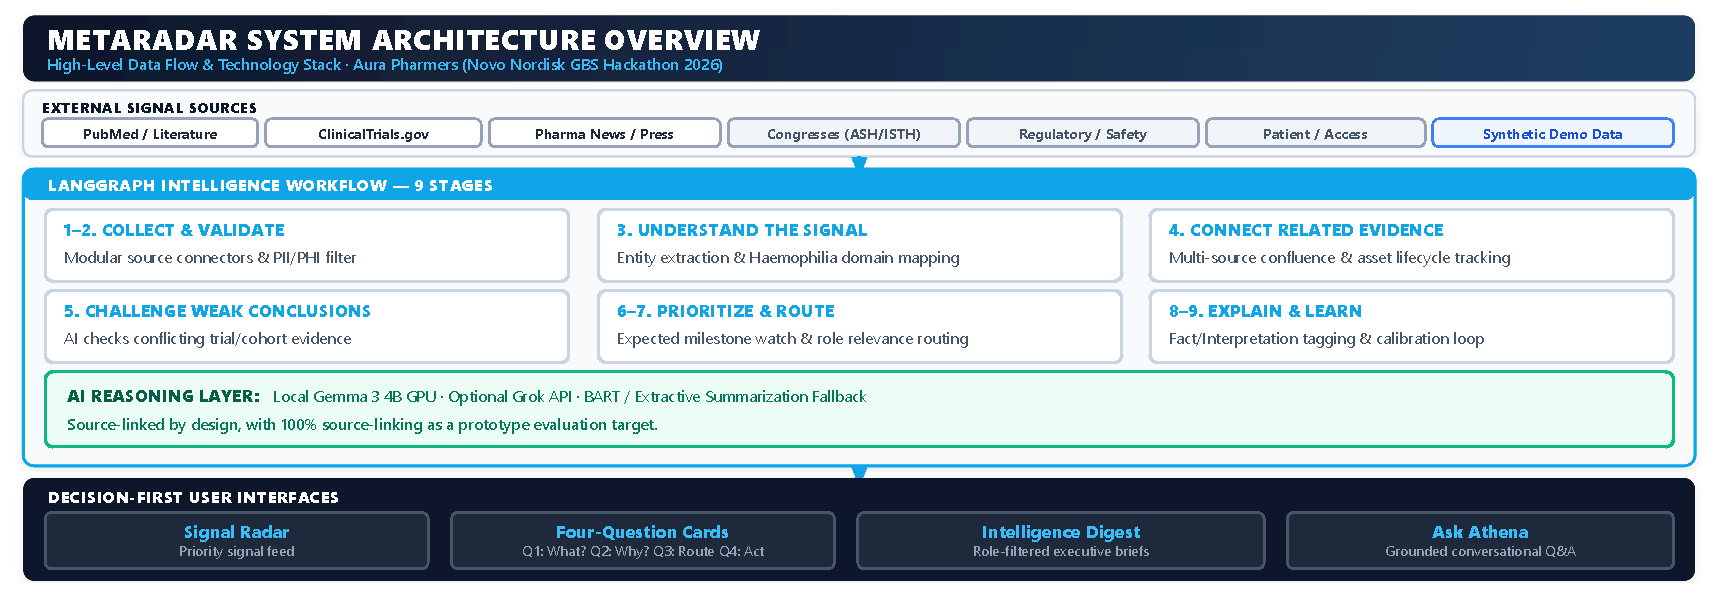
\includegraphics[width=0.96\textwidth]{architecture.pdf}
\captionof{figure}{\textbf{MetaRadar System Architecture} --- High-level data flow from public and synthetic sources through intelligence workflow and UI.}
\label{fig:architecture}
\end{center}

\clearpage

% ============================================================
% PAGE 2 — DIFFERENTIATION, CALIBRATION, TECHNOLOGY, TRUST & SCALE
% ============================================================

% ------------------------------------------------------------
% 6. DIFFERENTIATION
% ------------------------------------------------------------
\section{What Makes MetaRadar Different?}

MetaRadar is distinguished from conventional monitoring tools by \textbf{five core intelligence mechanisms}:

\begin{enumerate}[
    leftmargin=11pt,
    noitemsep,
    topsep=0.5pt
]

\item
\textbf{CONFLUENCE:}
Connects independent updates pointing to the same development within a rolling 48-hour window, so teams see one stronger intelligence story instead of several disconnected alerts.

\item
\textbf{LIFECYCLE:}
Shows how a development evolves over time across a clear progression: \textit{Announcement $\rightarrow$ Clinical Trial $\rightarrow$ Congress Readout $\rightarrow$ Publication $\rightarrow$ Regulatory Decision $\rightarrow$ Access Event $\rightarrow$ Post-Market Evidence}.

\item
\textbf{RED-TEAM:}
Challenges weak or unsupported AI interpretations by looking for conflicting evidence, population differences, endpoint mismatches, and other limitations that could change the interpretation.

\item
\textbf{WATCH-FOR-NEXT:}
Tracks developments that may require follow-up and watches for important future evidence or expected milestones, such as congress abstracts or regulatory developments.

\item
\textbf{STAKEHOLDER CALIBRATION:}
Compares AI baselines with expert feedback so relevance, urgency, routing, and suggested actions become more accurate and useful over time.

\end{enumerate}

% ------------------------------------------------------------
% CALIBRATION FIGURE
% ------------------------------------------------------------
\begin{center}
\vspace{-3pt}
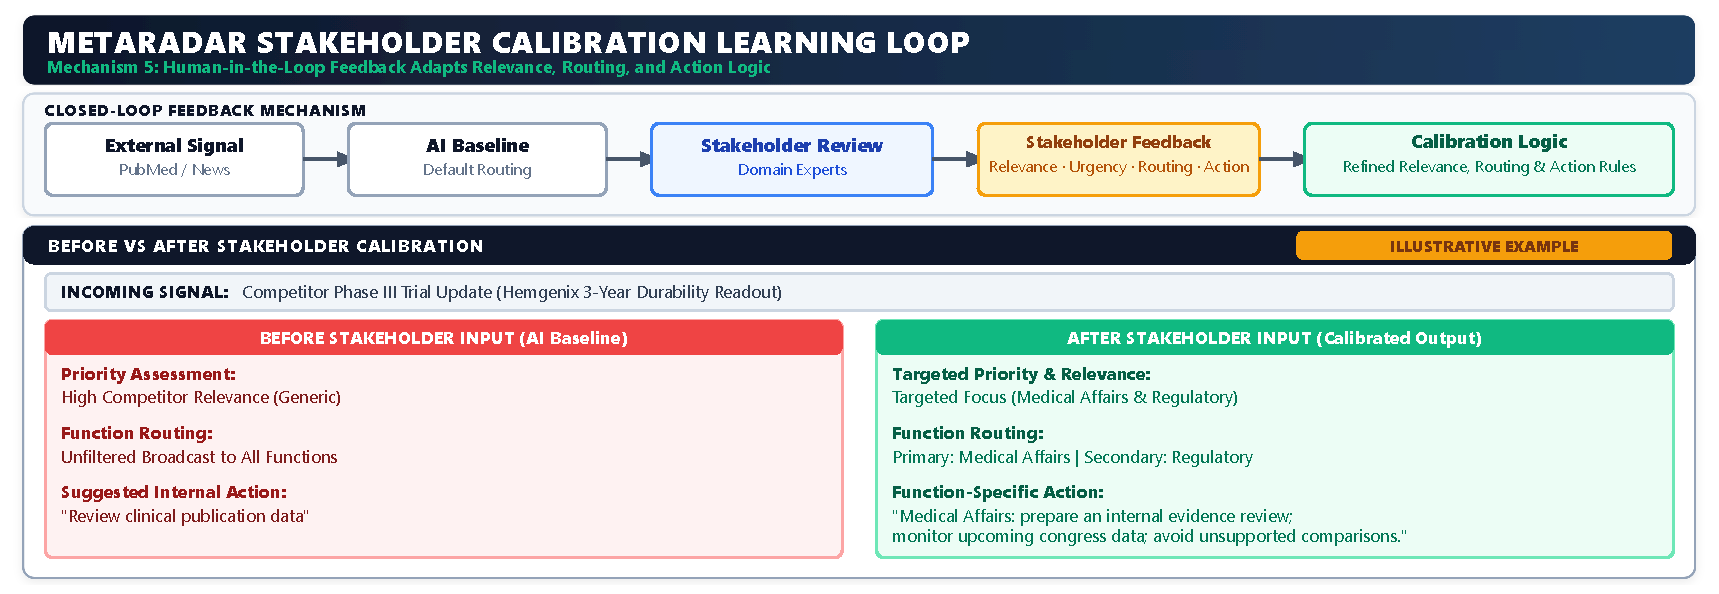
\includegraphics[width=0.96\textwidth]{stakeholder_calibration.pdf}
\captionof{figure}{\textbf{Stakeholder Calibration Learning Loop} --- Before vs.\ after stakeholder feedback for a competitor Phase III trial update (\textit{Illustrative Example}).}
\label{fig:calibration}
\end{center}

% ------------------------------------------------------------
% 7. TECHNOLOGY AT A GLANCE
% ------------------------------------------------------------
\section{Technology at a Glance}

\vspace{1pt}

{\scriptsize
\renewcommand{\arraystretch}{1.15}

\begin{tabularx}{\textwidth}{
    |>{\bfseries\color{NavyBlue}\raggedright\arraybackslash}p{2.8cm}
    |X|X|X|
}
\hline

\textbf{\color{NavyBlue}Category}
&
\textbf{\color{NavyBlue}Primary Component}
&
\textbf{\color{NavyBlue}Secondary / Hosted}
&
\textbf{\color{NavyBlue}Fallback / Utility}
\\
\hline

AI Reasoning
&
Gemma 3 4B (Local GPU)
&
xAI Grok API (Optional)
&
BART / Extractive Summarization Fallback
\\
\hline

Intelligence
&
Entity extraction \& evidence linking
&
Confluence \& lifecycle analysis
&
Red-Team \& stakeholder calibration
\\
\hline

Platform \& Infra
&
LangGraph / FastAPI
&
Next.js 15 UI
&
PostgreSQL / Redis 7
\\
\hline

Data Sources
&
PubMed Literature
&
ClinicalTrials.gov
&
NewsAPI / Regulatory
\\
\hline

\end{tabularx}
}

% ------------------------------------------------------------
% 8. SAFE BY DESIGN
% ------------------------------------------------------------
\section{Safe by Design}

\begin{itemize}[
    leftmargin=10pt,
    noitemsep
]

\item
Public, mock, or synthetic data only (zero confidential Novo Nordisk data and zero patient-identifiable PII/PHI).

\item
Every important insight remains linked to its supporting external source, evidence, and date.

\item
Each signal retains its source, publication/update date, and supporting evidence so users can trace an insight back to the underlying information.

\item
\textbf{FACT / INTERPRETATION / SPECULATION} are explicitly separated so assumptions are not presented as facts.

\item
Confidence reflects evidence strength, not medical certainty.

\item
AI suggests; human experts review and decide. High-impact safety, regulatory, and medical outputs require human review.

\end{itemize}

% ------------------------------------------------------------
% 9. DESIGNED TO SCALE
% ------------------------------------------------------------
\section{Designed to Scale}

Haemophilia is the pilot, not the limit of the platform. The core MetaRadar engine is separated from disease-specific knowledge, so another therapy area can reuse the same intelligence workflow while changing the relevant disease knowledge, terminology, sources, and routing rules.

% ------------------------------------------------------------
% 10. EVALUATION & EXPECTED OUTCOME
% ------------------------------------------------------------
\section{Prototype Evaluation \& Expected Outcome}

MetaRadar is evaluated against verifiable hackathon targets: \textbf{100\% source-linked summaries}, \textbf{$\geq$85\% classification accuracy}, \textbf{$\leq$5-minute discovery time} for top signals, \textbf{zero confidential/patient data}, and \textbf{demonstrable calibration improvement}.

\textbf{Expected Outcome:} MetaRadar transforms scattered external noise into clear strategic signal, empowering Novo Nordisk cross-functional teams to identify key developments faster, understand their significance, route them to the right function, and take informed internal action with confidence.

\end{document}
